\documentclass{article}


% Packages
\usepackage{fullpage}
\usepackage{amssymb}
\usepackage{multicol}
\usepackage{amsmath}
\usepackage{amsfonts}
\usepackage{bm}
\usepackage{float}
\usepackage{tikz}
\usepackage{xcolor}
\usetikzlibrary{shapes.geometric, positioning, arrows, intersections}
\usepackage{amsthm}
\usepackage{tcolorbox}
\usepackage{hyperref}
\hypersetup{
    colorlinks=true, %set true if you want colored links
    linktoc=all,     %set to all if you want both sections and subsections linked
    linkcolor=black,  %choose some color if you want links to stand out
}


% Macros
\newcommand{\R}{\mathbb{R}}
\newcommand{\N}{\mathbb{N}}
\newcommand{\Q}{\mathbb{Q}}
\newcommand{\sub}{\subset}
\renewcommand{\a}{\alpha}
\renewcommand{\b}{\beta}
\newcommand{\g}{\gamma}
\renewcommand{\d}{\delta}
\newcommand{\e}{\varepsilon}
\newcommand{\ex}{\exists\,}
\newcommand{\overbar}[1]{\mkern 1.5mu\overline{\mkern-1.5mu#1\mkern-1.5mu}\mkern 1.5mu}
\newcommand{\eR}{\overbar{\R}}

%\setlength{\columnsep}{20pt}

%ToC stuff
\newtheorem{example}{Example}
\newtheorem{solution}{Solution}
%\newtheorem{definition}{Definition}[subsection]
\newtheorem{corollary}{Corollary}

\tcbuselibrary{theorems}
\newtcbtheorem[number within=section]{theorem}{Theorem}%
{colback=green!5,colframe=green!35!black,fonttitle=\bfseries}{th}
\newtcbtheorem[number within=section]{definition}{Definition}%
{colback=blue!5,colframe=blue!35!black,fonttitle=\bfseries}{def}

 % Document stuff

\title{Week 2: Limits and Functions}
\author{James Arthur}

\begin{document}
\maketitle
\tableofcontents
\newpage

\multicols{2}


\section{Overview}

The reals ($\R$) have a few properties:
\begin{enumerate}
  \item They are a field, i.e. a groupoid with {\color{blue}two binary operations}.
  \item They are ordered
  \item They are also {\color{blue}complete}.
\end{enumerate}
We will also look at {\color{blue}supremum} and the {\color{blue}infimum}.

We are also going to look at the {\color{blue}extended real numbers}. We are going to add two more fictitious points. $\R \cup \{ \infty \} \cup \{ -\infty \}$.

\section{Properties of the Reals}
We will be taking the axiomatic view point of the real numbers. No construction with {\color{blue}Dedekind cuts} or {\color{blue}Cauchy sequences}. All of these are isomorphic.

\subsection{Field Properties}
The real numbers are a set, $\R$, with two binary operations, $+$ and $\times$. They must satisfy the following axioms. So take $a, b, c \in \R$:
\begin{enumerate}
  \item $a + b = b + a$ and $ab = ba$ ({\color{blue}commutativity})
  \item $(a + b) + c = a + (b + c)$ and $a(bc) = (ab)c$ ({\color{blue}associativity})
  \item $a(b + c) = ab + ac$ ({\color{blue}distributivity})
  \item There are two distinctive identities $0$ ({\color{blue}additive identity}) and $1$ ({\color{blue}multiplicative identity}), such that $a + 0 = 0 + a = a$ and $a1 = 1a = a$
  \item We also have inverses, $-a$ ({\color{blue}additive inverse}) such that $a + -a = 0$ and if $a \neq 0$, there is a real number $\frac{1}{a}$ such that: $a(\frac{1}{a})=1$
\end{enumerate}

\subsection{Order Relation}

The real numbers are {\color{blue}ordered}, that means:
\begin{enumerate}
  \item For each pair of reals $a$ and $b$, exactly one of the following is true
  $$ a = b \qquad a < b \qquad b < a $$
  \item It is also {\color{blue}transitive}, if $a < b$ and $b < c$, then $a < c$
  \item If $a < b$ then $a + c < b + c$ for any $c$, and if $0 < c$, then $ac < bc$
\end{enumerate}

\subsection{Supremum}

Let $S\sub \R$. If there exists $b\in\R$ such that $x \le b \quad\forall x\in S$ then $S$ is {\color{blue}bounded above} and $b$ is an {\color{blue}upper bound of $S$}.

If $\b$ is an upper bound of $S$, but no number less than $\b$ is, then $\b$ is called the {\color{blue}supremum} of S, denoted:
$$ \b = \sup S $$
\vspace{-10pt}
\begin{figure}[H]
  \centering
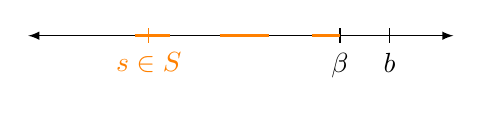
\begin{tikzpicture}[scale=0.9]
\draw[latex-latex] (-3,0) -- (3,0) ; %edit here for the axis
\draw[shift={(2.1,0)},color=black] (0pt,3pt) -- (0pt,-3pt);
\draw[shift={(2.1,0)},color=black] (0pt,0pt) -- (0pt,-3pt) node[below]
{$b$};
\draw[shift={(1.4,0)},color=black] (0pt,3pt) -- (0pt,-3pt);
\draw[shift={(1.4,0)},color=black] (0pt,0pt) -- (0pt,-3pt) node[below]
{$\b$};
\draw[shift={(-1.3,0)},color=orange] (0pt,3pt) -- (0pt,-3pt);
\draw[shift={(-1.3,0)},color=orange] (0pt,0pt) -- (0pt,-3pt) node[below]
{$s\in S$};
\draw[very thick, color=orange] (1,0) -- (1.4,0);
\draw[very thick, color=orange] (-1.5,0) -- (-1,0);
\draw[very thick, color=orange] (-0.3,0) -- (0.4,0);
\end{tikzpicture}
\caption{\textit{Let $S$ be the orange set and then $b$ is an upper bound of S and $\b$ is $\sup S$}}
\end{figure}
We also call the supremum the least upper bound.\\
\begin{example}{
  $S = [\,0, 1\,]$ and prove $sup\, S = 1$
}\end{example}
\begin{figure}[H]
  \centering
\begin{tikzpicture}[scale=0.9]
\draw[latex-latex] (-3,0) -- (3,0) ; %edit here for the axis
\draw[shift={(0,0)},color=black] (0pt,3pt) -- (0pt,-3pt);
\draw[shift={(0,0)},color=black] (0pt,0pt) -- (0pt,-3pt) node[below]
{$0$};
\draw[shift={(1,0)},color=black] (0pt,3pt) -- (0pt,-3pt);
\draw[shift={(1,0)},color=black] (0pt,0pt) -- (0pt,-3pt) node[below]
{$1$};
\draw[very thick, color=green] (0,0) -- (1,0);
\end{tikzpicture}
\end{figure}
\begin{solution}
Take our diagram from above,
We need to check that $x \le 1 \quad\forall\, x \in S$, which is definitionally true.\\
Secondly we need to prove that $\forall\, b < 1,\: \ex\, x \in S, \,b < x$, which is again trivially true. So $\sup S = 1$
\end{solution}\vspace{10pt}
\begin{example}{
 Take $T = (\,0, 1\,)$ where $\sup T = 1$
}\end{example}\begin{solution}{
  Again every number is less than 1, but if you take any number less than one you can always find another element larger.\\
  {\color{red} \textbf{NB: The supremum here isn't in the set}}
}\end{solution}\vspace{10pt}

\subsection{Infimum}
Similarly, if there exists an $a \in \R$ such that $a \le x \quad x \in S$, then $S$ is {\color{blue}bounded below} and $a$ is a {\color{blue}lower bound of $S$}.\\

If $\a$ is a lower bound of $S$, but no number is greater than $\a$ is, then $\a$ is called the {\color{blue} infimum } of $S$:
$$ \a = \inf \, S $$
\vspace{-30pt}
\begin{figure}[H]
  \centering
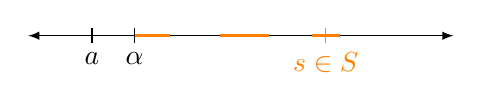
\begin{tikzpicture}[scale=0.9]
\draw[latex-latex] (-3,0) -- (3,0) ; %edit here for the axis
\draw[shift={(-2.1,0)},color=black] (0pt,3pt) -- (0pt,-3pt);
\draw[shift={(-2.1,0)},color=black] (0pt,0pt) -- (0pt,-3pt) node[below]
{$a$};
\draw[shift={(-1.5,0)},color=black] (0pt,3pt) -- (0pt,-3pt);
\draw[shift={(-1.5,0)},color=black] (0pt,0pt) -- (0pt,-3pt) node[below]
{$\a$};
\draw[shift={(1.2,0)},color=orange] (0pt,3pt) -- (0pt,-3pt);
\draw[shift={(1.2,0)},color=orange] (0pt,0pt) -- (0pt,-3pt) node[below]
{$s\in S$};
\draw[very thick, color=orange] (1,0) -- (1.4,0);
\draw[very thick, color=orange] (-1.5,0) -- (-1,0);
\draw[very thick, color=orange] (-0.3,0) -- (0.4,0);
\end{tikzpicture}
\caption{\textit{Let $S$ be the orange set and then $a$ is a lower bound of S and $\a$ is $\inf\, S$}}
\end{figure}
Another name for the infimum is the greatest lower bound.

\subsection{Completeness Axiom}

Do the supremum and the infimum actually exist? Well, not all subsets are bounded above, i.e. $\R \sub \R$ or what about the empty set? This is what the completeness axiom does:
\begin{enumerate}
  \item If a non-empty set of real numbers are bounded above, then it has a supremum.
\end{enumerate}

So the reals are a {\color{red} \textbf{complete ordered field} }\\

The completeness axiom is distinguishing of the reals. They are the only complete ordered field. The rationals possess everything but completeness in terms of our axioms.\\

\noindent
\begin{example}
 We restrict to the $\Q,\quad S = \{ r \in \Q : r^2 < 2 \} $. Find the supremum and infimum.
\end{example}\begin{solution}
If we take the example below;
\begin{figure}[H]
  \centering
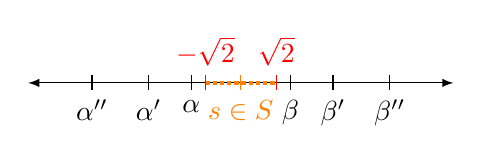
\begin{tikzpicture}[scale=0.9]
\draw[latex-latex] (-3,0) -- (3,0) ; %edit here for the axis
\draw[densely dotted, ultra thick, orange] (-0.5,0) -- (0.5,0); % adds a dotted line
\draw[shift={(-2.1,0)},color=black] (0pt,3pt) -- (0pt,-3pt);
\draw[shift={(-2.1,0)},color=black] (0pt,0pt) -- (0pt,-3pt) node[below]
{$\a''$};
\draw[shift={(-1.3,0)},color=black] (0pt,3pt) -- (0pt,-3pt);
\draw[shift={(-1.3,0)},color=black] (0pt,0pt) -- (0pt,-3pt) node[below]
{$\a'$};
\draw[shift={(-0.7,0)},color=black] (0pt,3pt) -- (0pt,-3pt);
\draw[shift={(-0.7,0)},color=black] (0pt,0pt) -- (0pt,-3pt) node[below]
{$\a$};
\draw[shift={(2.1,0)},color=black] (0pt,3pt) -- (0pt,-3pt);
\draw[shift={(2.1,0)},color=black] (0pt,0pt) -- (0pt,-3pt) node[below]
{$\b''$};
\draw[shift={(1.3,0)},color=black] (0pt,3pt) -- (0pt,-3pt);
\draw[shift={(1.3,0)},color=black] (0pt,0pt) -- (0pt,-3pt) node[below]
{$\b'$};
\draw[shift={(0.7,0)},color=black] (0pt,3pt) -- (0pt,-3pt);
\draw[shift={(0.7,0)},color=black] (0pt,0pt) -- (0pt,-3pt) node[below]
{$\b$};
\draw[shift={(0,0)},color=orange] (0pt,3pt) -- (0pt,-3pt);
\draw[shift={(0,0)},color=orange] (0pt,0pt) -- (0pt,-3pt) node[below]
{$s\in S$};
\draw[shift={(0.5,0)},color=red] (0pt,3pt) -- (0pt,-3pt);
\draw[shift={(0.5,0)},color=red] (0pt,0pt) -- (0pt,3pt) node[above]
{$\sqrt 2$};
\draw[shift={(-0.5,0)},color=red] (0pt,3pt) -- (0pt,-3pt);
\draw[shift={(-0.5,0)},color=red] (0pt,0pt) -- (0pt,3pt) node[above]
{$-\sqrt 2$};
\end{tikzpicture}
\end{figure}

we can say that we won't reach $\sqrt 2$ in the supremum or $-\sqrt 2$ in the infimum. This is because we are using rationals and $\sqrt 2$ is an irrational. We can go either way and there is always a number closer to $\sqrt 2$.\\

This proves that rationals are not complete.

\end{solution}\vspace{10pt}

\section{Extended Real Numbers}
It is convenient to attach $\infty$ and $-\infty$ to the reals. How do they fit in? Firstly lets look at orders. Take $x\in \R$, then:
$$ -\infty < x <\infty $$
Now if a set $S$ is unbounded above or below, we can write:
$$ \sup\, S =\infty \quad \inf\, S = -\infty $$

\begin{example}
 Find the infimum of $S = \{ x\in \R : x : 2 \}$
\end{example}\begin{solution}{
\begin{figure}[H]
  \centering
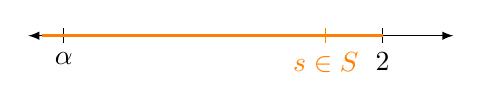
\begin{tikzpicture}[scale=0.9]
\draw[latex-latex] (-3,0) -- (3,0) ; %edit here for the axis
\draw[shift={(2,0)},color=black] (0pt,3pt) -- (0pt,-3pt);
\draw[shift={(2,0)},color=black] (0pt,0pt) -- (0pt,-3pt) node[below]
{$2$};
\draw[shift={(-2.5,0)},color=black] (0pt,3pt) -- (0pt,-3pt);
\draw[shift={(-2.5,0)},color=black] (0pt,0pt) -- (0pt,-3pt) node[below]
{$\a$};
\draw[shift={(1.2,0)},color=orange] (0pt,3pt) -- (0pt,-3pt);
\draw[shift={(1.2,0)},color=orange] (0pt,0pt) -- (0pt,-3pt) node[below]
{$s\in S$};
\draw[very thick, color=orange] (-2.8,0) -- (2,0);
\end{tikzpicture}
\end{figure}
  As there is technically no lower bound, it is $-\infty$
}\end{solution}\vspace{10pt}

We usually denote the extended reals with the symbol, $\overbar{\R} $ or $[-\infty, \infty]$ or $\R \cup \{-\infty, \infty \}$


\subsection{Arithmetic}
If $a \in \R$,
\begin{enumerate}
  \item Then:
  \begin{align*}
    a + \infty &= \infty + a = \infty\\
    a - \infty &= -\infty + a = -\infty\\
    \frac{a}{\infty} &= \frac{a}{-\infty} = 0\\
  \end{align*}
  \item and $0 < a$, then:
  \begin{align*}
    a\infty &= \infty a = \infty \\
    a(-\infty) &= (-\infty)a = -\infty\\
  \end{align*}
  \item and $a < 0$, then:
  \begin{align*}
    a\infty &= \infty a = -\infty\\
    a(-\infty) &= (-\infty)a = \infty\\
  \end{align*}
\end{enumerate}

We also define:
\begin{enumerate}
  \item $\infty + \infty = \infty\infty = (-\infty)(-\infty) = \infty$\\
  \item and also $- \infty - \infty = \infty(-\infty) = (-\infty)\infty = -\infty$\\
  \item and finally, $|\infty| = |-\infty| = \infty$
\end{enumerate}

We say it isn't useful to define; $\infty - \infty$, $0 \cdot \infty$, $\displaystyle{\frac{\infty}{\infty}}$ and $\displaystyle{\frac{0}{0}}$. We call them indeterminate forms.

\section{Triangle Inequality}
As we can use the ordered relation of the reals we can produce something known as the {\color{blue} triangle inequality}.
\begin{theorem}{Triangle Inequality}{}
  It states for any $a, b \in \R$, we have:
  $$ |a + b| \le |a| + |b|$$
\end{theorem}
\begin{proof}
  There are four possibilities:
  \begin{enumerate}
    \item If $0 \le a$ and $0 \le b$, then $0 \le a + b$, so $|a + b| = a + b = |a| + |b|$.
    \item If $a \le 0$ and $b \le 0$, then $a + b \le 0$, so $|a + b| = -a + (-b) = |a| + |b|$.
    \item If $0 \le a$ and $b \le 0$, then $a + b = |a| - |b|$.
    \item If $a \le 0$ and $0 \le b$, then $a + b = -|a| + |b|$.
  \end{enumerate}

It holds in cases (c) and (d), since
$$ ||a| - |b|| = \begin{cases}
|a| - |b| & \text{ if } |b| \le |a|,\vspace{5px}\\
|b| - |a| & \text{ if } |a| \le |b|.\\
\end{cases}
 $$
\end{proof}

\section{Open and Closed Sets}
\begin{definition}
  We define an {\color{blue} open interval} between $\displaystyle{a}$ and $\displaystyle{b}$, $\displaystyle{a, b \in \eR}$, as such:
  $$ (a,\, b) = \{ x: a < x < b\} $$
  \end{definition}
  \begin{figure}[H]
    \centering
    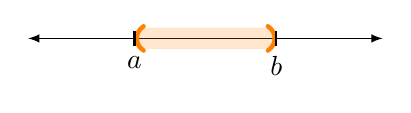
\begin{tikzpicture}[scale=0.9]
  \draw[latex-latex] (-1.5,0) -- (3.5,0) ; %edit here for the axis
  \draw[(-, ultra thick, orange] (0,0) -- (0.01,0);
  \draw[-), ultra thick, orange] (2,0) -- (2.01,0);
  \fill[opacity = 0.2, orange, rounded corners=1ex] (0,-1ex) -- (2, -1ex) -- (2, 1ex) -- (0,1ex) -- cycle;
  \draw[shift={(0,0)}, thick, color=black] (0pt,3pt) -- (0pt,-3pt);
  \draw[shift={(0,0)}, thick, color=black] (0pt,0pt) -- (0pt,-3pt) node[below]
  {$a$};
  \draw[shift={(2,0)}, thick, color=black] (0pt,3pt) -- (0pt,-3pt);
  \draw[shift={(2,0)}, thick, color=black] (0pt,0pt) -- (0pt,-3pt) node[below]
  {$b$};
  \end{tikzpicture}
  \end{figure}

\begin{definition}
  We define a {\color{blue} closed interval} between $\displaystyle{a}$ and $\displaystyle{b}$, $\displaystyle{a, b \in \eR}$, as such:
  $$ [a,\, b] = \{ x: a \le x \le b \} $$
  \end{definition}
  \begin{figure}[H]
    \centering
    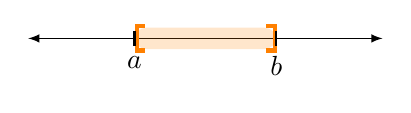
\begin{tikzpicture}[scale=0.9]
  \draw[latex-latex] (-1.5,0) -- (3.5,0) ; %edit here for the axis
  \draw[[-, ultra thick, orange] (0,0) -- (0.01,0);
  \draw[{-]}, ultra thick, orange] (2,0) -- (2.01,0);
  \fill[opacity = 0.2, orange, rounded corners=1ex] (0,-1ex) -- (2, -1ex) -- (2, 1ex) -- (0,1ex) -- cycle;
  \draw[shift={(0,0)}, thick, color=black] (0pt,3pt) -- (0pt,-3pt);
  \draw[shift={(0,0)}, thick, color=black] (0pt,0pt) -- (0pt,-3pt) node[below]
  {$a$};
  \draw[shift={(2,0)}, thick, color=black] (0pt,3pt) -- (0pt,-3pt);
  \draw[shift={(2,0)}, thick, color=black] (0pt,0pt) -- (0pt,-3pt) node[below]
  {$b$};
  \end{tikzpicture}
  \end{figure}

\subsection{Neightbourhoods}

A neighborhood is used to talk about closeness of points. We are now going to go through a load of set definitions!\\

\begin{definition}{}{}
 If $\displaystyle{x_0}$ is a real number and $\displaystyle{\e>0}$, then the open interval $\displaystyle{(x_0 - \e, x_0 + \e)}$ is an {\color{blue} $\e$-neighbourhood of $x_0$}.
\end{definition}\vspace{10pt}
 \begin{figure}[H]
   \centering
   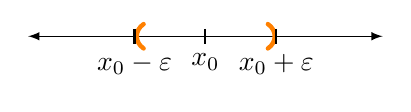
\begin{tikzpicture}[scale=0.9]
     \draw[latex-latex] (-1.5,0) -- (3.5,0) ; %edit here for the axis
     \draw[(-, ultra thick, orange] (0,0) -- (0.01,0);
     \draw[{-)}, ultra thick, orange] (2,0) -- (2.01,0);
     %\fill[opacity = 0.2, blue,rounded corners=1ex] (0,-1ex) -- (2, -1ex) -- (2, 1ex) -- (0,1ex) -- cycle;
     \draw[shift={(0,0)}, thick, color=black] (0pt,3pt) -- (0pt,-3pt);
     \draw[shift={(0,0)}, thick, color=black] (0pt,0pt) -- (0pt,-3pt) node[below]
     {$x_0 - \e$};
     \draw[shift={(2,0)}, thick, color=black] (0pt,3pt) -- (0pt,-3pt);
     \draw[shift={(2,0)}, thick, color=black] (0pt,0pt) -- (0pt,-3pt) node[below]
     {$x_0 + \e$};
     \draw[shift={(1,0)}, thick, color=black] (0pt,3pt) -- (0pt,-3pt);
     \draw[shift={(1,0)}, thick, color=black] (0pt,0pt) -- (0pt,-3pt) node[below]
     {$x_0$};
   \end{tikzpicture}
 \end{figure}


\begin{definition}{}{}
 If a set $S$ contains an $\e$-neighbourhood of $x_0$, then $S$ is a {\color{blue} neighborhood of $x_0$}. i.e. we need $\displaystyle{(x_0-\e,\, x_0+\e) \sub S}$
\end{definition}\vspace{10pt}
 \begin{figure}[H]
   \centering
   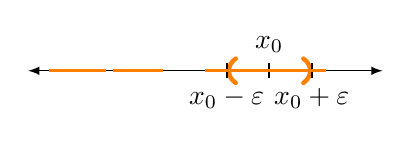
\begin{tikzpicture}[scale=0.9]
     \draw[latex-latex] (-1.5,0) -- (3.5,0) ; %edit here for the axis
     \draw[(-, ultra thick, orange] (1.3,0) -- (1.31,0);
     \draw[{-)}, ultra thick, orange] (2.5,0) -- (2.51,0);
     %\fill[opacity = 0.2, blue,rounded corners=1ex] (0,-1ex) -- (2, -1ex) -- (2, 1ex) -- (0,1ex) -- cycle;
     \draw[shift={(1.3,0)}, thick, color=black] (0pt,3pt) -- (0pt,-3pt);
     \draw[shift={(1.3,0)}, thick, color=black] (0pt,0pt) -- (0pt,-3pt) node[below]
     {$x_0 - \e$};
     \draw[shift={(2.5,0)}, thick, color=black] (0pt,3pt) -- (0pt,-3pt);
     \draw[shift={(2.5,0)}, thick, color=black] (0pt,0pt) -- (0pt,-3pt) node[below]
     {$x_0 + \e$};
     \draw[shift={(1.9,0)}, thick, color=black] (0pt,3pt) -- (0pt,-3pt);
     \draw[shift={(1.9,0)}, thick, color=black] (0pt,0pt) -- (0pt,3pt) node[above]
     {$x_0$};
     \draw[very thick, color=orange] (1,0) -- (2.7,0);
     \draw[very thick, color=orange] (-1.2,0) -- (-0.4,0);
     \draw[very thick, color=orange] (-0.3,0) -- (0.4,0);
   \end{tikzpicture}
 \end{figure}

\begin{definition}{}{}
 If $S$ is a neighbourhood of $x_0$, then $x_0$ is an {\color{blue} interior point of $S$}.
\end{definition}\vspace{10pt}
 \begin{figure}[H]
   \centering
   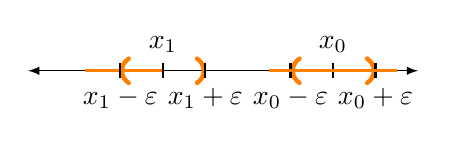
\begin{tikzpicture}[scale=0.9]
     \draw[latex-latex] (-2,0) -- (3.5,0) ; %edit here for the axis
     \draw[(-, ultra thick, orange] (1.7,0) -- (1.71,0);
     \draw[{-)}, ultra thick, orange] (2.9,0) -- (2.91,0);
     %\fill[opacity = 0.2, blue,rounded corners=1ex] (0,-1ex) -- (2, -1ex) -- (2, 1ex) -- (0,1ex) -- cycle;
     \draw[shift={(1.7,0)}, thick, color=black] (0pt,3pt) -- (0pt,-3pt);
     \draw[shift={(1.7,0)}, thick, color=black] (0pt,0pt) -- (0pt,-3pt) node[below]
     {$x_0 - \e$};
     \draw[shift={(2.9,0)}, thick, color=black] (0pt,3pt) -- (0pt,-3pt);
     \draw[shift={(2.9,0)}, thick, color=black] (0pt,0pt) -- (0pt,-3pt) node[below]
     {$x_0 + \e$};
     \draw[shift={(2.3,0)}, thick, color=black] (0pt,3pt) -- (0pt,-3pt);
     \draw[shift={(2.3,0)}, thick, color=black] (0pt,0pt) -- (0pt,3pt) node[above]
     {$x_0$};
     %
     \draw[very thick, color=orange] (1.4,0) -- (3.2,0);
     \draw[very thick, color=orange] (-1.2,0) -- (-0.4,0);
     \draw[very thick, color=orange] (-0.8,0) -- (-0.1,0);
     %
     \draw[-), ultra thick, orange] (0.5,0) -- (0.51,0);
     \draw[{-)}, ultra thick, orange] (-0.7,0) -- (-0.71,0);
     \draw[shift={(-0.7,0)}, thick, color=black] (0pt,3pt) -- (0pt,-3pt);
     \draw[shift={(-0.7,0)}, thick, color=black] (0pt,0pt) -- (0pt,-3pt) node[below]
     {$x_1 - \e$};
     \draw[shift={(0.5,0)}, thick, color=black] (0pt,3pt) -- (0pt,-3pt);
     \draw[shift={(0.5,0)}, thick, color=black] (0pt,0pt) -- (0pt,-3pt) node[below]
     {$x_1 + \e$};
     \draw[shift={(-0.1,0)}, thick, color=black] (0pt,3pt) -- (0pt,-3pt);
     \draw[shift={(-0.1,0)}, thick, color=black] (0pt,0pt) -- (0pt,3pt) node[above]
     {$x_1$};
   \end{tikzpicture}
   \caption{$x_0$ is an interior point, however $x_1$ is not}
 \end{figure}

\begin{definition}{}{}
 The set of interior points of $S$ is the {\color{blue} interior } of $S$, denoted by {\color{blue} $S^0$ }
\end{definition}\vspace{10pt}

\begin{definition}{Interior Point}{}
 If every point of S is an interior point, ($S^0 = S$), then $S$ is {\color{blue} open }.
\end{definition}\vspace{10pt}

\begin{definition}{}{}
 A set is {\color{blue} closed } if $S^c$ is open.
\end{definition}\vspace{10pt}

\begin{example}{
 Any open interval $S= (a,\,b)$ is open.\\
}\end{example}\begin{solution}{
Need to show that $\displaystyle{\forall x_0\in(a,\, b), \: \ex \e>0: (x_0 - \e, x_0+\e)\sub (a,\,b)}$\\
Assume that $\displaystyle{a, b \in \R}$. Let $\displaystyle{x_0\in(a,\,b)}$ and let $\e = \min (x_0 - a, b - x_0)$. Then clearly $\displaystyle{(x_0-\e,\, x_0+\e)\sub (a,\, b)}$. \\
The rest of the proof is left as an exercise. (Where $a = -\infty$ or $b=\infty$).\\
Now we know that $\R$ is open and $S^c$, where $S^c = (-\infty,\, a)\cup[b, \infty)$, and $\varnothing$ is closed
}\end{solution}\vspace{10pt}

We also note that because of a vacouity argument $\varnothing$ is also open, hence $\displaystyle{\R}$ is also closed. So $\displaystyle{\R}$ and $\displaystyle{\varnothing}$ are both open and closed.

\subsection{Unions and Intersections}

\begin{theorem}{Unions and Intersection of closed and open sets}{}
  \begin{enumerate}
    \item  The union of open sets is open
    \item The intersection of closed sets is closed
  \end{enumerate}
  These apply to abtritary collections (finite or infinite of open and closed sets).
\end{theorem}
\begin{proof}
  First lets prove (1), so let $\displaystyle{\mathcal{G}}$ be a collection of open sets.\\
  Let $\displaystyle{S = \bigcup_{G \in \mathcal{G}}G}$, If $\displaystyle{x_0 \in S}$, then $\displaystyle{x_0 \in G_0}$ for some $\displaystyle{G_0 \in \mathcal{G}}$. Since $G_0$ is open, it must contain an $\e$- neighborhood of $x_0$. The $\e$-neighborhood, $(x_0-\e, x_0+\e)$, is in $S$, hence $S$ is a neighborhood of $x_0$ and $x_0$ is an interior point of S. \\
  Since $x_0$ was arbitrary, then all points in $S$ are interior points and hence, $S$ is open.\\
  Now for part (2) of the theorem. Let $\displaystyle{\mathcal{F}}$ be a collection of closed sets and let $\displaystyle{T = \bigcap_{F\in \mathcal{F}}F}$. Then $\displaystyle{T^c = \bigcup_{F\in\mathcal{F}}F^c}$. Since each $F^c$ is open, that means $T^c$ is open by (1). Therefore $T$ is closed
\end{proof}

\begin{example}{
 For $a, b \in \R$, the sets $[a,\, b]$ is closed.
}\end{example}\begin{solution}{
  Since $[a,\, b]^c = (-\infty,\, a) \cup (b, \infty)$. Since its a union of open intervals, it is open. Hence making $[a,\, b]$ closed.
}\end{solution}\vspace{10pt}

\begin{example}{
  What about $[a, b)$, or $(a, b]$ for $a, b \in \R$?
}\end{example}\begin{solution}{
  These are half-open or half-closed intervals. These are neither open nor closed. Take $\displaystyle{[a,\, b)}$, then $a$ isn't an interior point of the set, hence it's not open. Now take the compliment of the set $\displaystyle{[a,\,b)^c = (-\infty,\, a)\cup[b,\, \infty)}$ and now $b$ is no longer an interior point. Hence, not closed.
}\end{solution}\vspace{10pt}

\begin{example}{
 What about: $\displaystyle{(-\infty,\,a]}$ or $\displaystyle{[a,\,\infty)}$
}\end{example}\begin{solution}{
  Exercise
}\end{solution}\vspace{10pt}

Now, what about the intersection of open sets and union of closed sets. Well, it can be proved that the intersection of finitely many open sets is open and union of finitely many closed sets is closed. However the infinite versions of these statements need not be the same.

{\color{red} \textbf{The concept of open and closed sets, doesn't form a dichotomy (A set is partitioned into two. i.e. odd or even naturals). }} A set can be neither open or closed or both.\\

\begin{definition}{}{}
 A {\color{blue} deleted neighbourhood } of a point $\displaystyle{x_0}$ is a set that contains every point of some neighborhood of $\displaystyle{x_0}$ except $\displaystyle{x_0}$. For example:
 $$ S = \{x : 0 < |x - x_0| < \e \} $$
 is a deleted neighborhood of $x_0$. We also say it is deleted $\e$-neighborhood of $x_0$.
\end{definition}\vspace{10pt}

Let $S$ be a subset of $\R$.

\begin{definition}{}{}
  $x_0$ is a {\color{blue} limit point } of $S$ if every deleted neighbourhood of $x_0$ contains a point of $S$
\end{definition}\vspace{10pt}

\begin{example}{
  Let $S = (-\infty,\,-1] \cup (1,\, 2) \cup \{3\}$. Find the limit points of $S$.
}\end{example}\begin{solution}{

\begin{figure}[H]
  \centering
  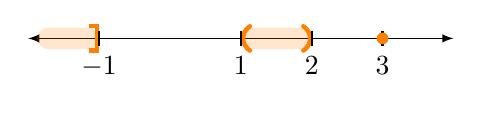
\begin{tikzpicture}[scale=0.9]
\draw[latex-latex] (-2,0) -- (4,0) ; %edit here for the axis
\draw[{[-}, ultra thick, orange] (-1,0) -- (-1.01,0);
\fill[opacity = 0.2, orange, rounded corners=1ex] (-1.88,-1ex) -- (-1, -1ex) -- (-1, 1ex) -- (-1.88,1ex) -- cycle;
\draw[shift={(-1,0)}, thick, color=black] (0pt,3pt) -- (0pt,-3pt);
\draw[shift={(-1,0)}, thick, color=black] (0pt,0pt) -- (0pt,-3pt) node[below]
{$-1$};
%
\draw[(-, ultra thick, orange] (1,0) -- (1.01,0);
\draw[-), ultra thick, orange] (2,0) -- (2.01,0);
\fill[opacity = 0.2, orange, rounded corners=1ex] (1,-1ex) -- (2, -1ex) -- (2, 1ex) -- (1,1ex) -- cycle;
\draw[shift={(1,0)}, thick, color=black] (0pt,3pt) -- (0pt,-3pt);
\draw[shift={(1,0)}, thick, color=black] (0pt,0pt) -- (0pt,-3pt) node[below]
{$1$};
\draw[shift={(2,0)}, thick, color=black] (0pt,3pt) -- (0pt,-3pt);
\draw[shift={(2,0)}, thick, color=black] (0pt,0pt) -- (0pt,-3pt) node[below]
{$2$};
%
\draw[shift={(3,0)}, thick, color=black] (0pt,3pt) -- (0pt,-3pt);
\draw[shift={(3,0)}, thick, color=black] (0pt,0pt) -- (0pt,-3pt) node[below]
{$3$};
\node at (3,0) [circle,fill,inner sep=1.5pt, color=orange]{};
\end{tikzpicture}
\end{figure}

Every point in $S$ is limit point, apart from $\{3 \}$
}\end{solution}\vspace{10pt}

\begin{definition}{}{}
  $\displaystyle{x_0}$ is a {\color{blue} boundary point } of $S$ if every neighborhood of $\displaystyle{x_0}$ contains at least one point in $S$ and one not in $S$. The set of boundary points of $S$  is the {\color{blue} boundary } of $S$, denoted by $\partial S$. The {\color{blue} closure } of $S$, denoted by $\overline S$, is $\overline S = S \cup \partial S$
\end{definition}\vspace{10pt}

\begin{example}{
  Let $S = (-\infty,\,-1] \cup (1,\, 2) \cup \{3\}$. Find the closure of $S$.
}\end{example}\begin{solution}{

\begin{figure}[H]
  \centering
  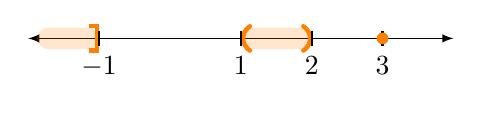
\begin{tikzpicture}[scale=0.9]
\draw[latex-latex] (-2,0) -- (4,0) ; %edit here for the axis
\draw[{[-}, ultra thick, orange] (-1,0) -- (-1.01,0);
\fill[opacity = 0.2, orange, rounded corners=1ex] (-1.88,-1ex) -- (-1, -1ex) -- (-1, 1ex) -- (-1.88,1ex) -- cycle;
\draw[shift={(-1,0)}, thick, color=black] (0pt,3pt) -- (0pt,-3pt);
\draw[shift={(-1,0)}, thick, color=black] (0pt,0pt) -- (0pt,-3pt) node[below]
{$-1$};
%
\draw[(-, ultra thick, orange] (1,0) -- (1.01,0);
\draw[-), ultra thick, orange] (2,0) -- (2.01,0);
\fill[opacity = 0.2, orange, rounded corners=1ex] (1,-1ex) -- (2, -1ex) -- (2, 1ex) -- (1,1ex) -- cycle;
\draw[shift={(1,0)}, thick, color=black] (0pt,3pt) -- (0pt,-3pt);
\draw[shift={(1,0)}, thick, color=black] (0pt,0pt) -- (0pt,-3pt) node[below]
{$1$};
\draw[shift={(2,0)}, thick, color=black] (0pt,3pt) -- (0pt,-3pt);
\draw[shift={(2,0)}, thick, color=black] (0pt,0pt) -- (0pt,-3pt) node[below]
{$2$};
%
\draw[shift={(3,0)}, thick, color=black] (0pt,3pt) -- (0pt,-3pt);
\draw[shift={(3,0)}, thick, color=black] (0pt,0pt) -- (0pt,-3pt) node[below]
{$3$};
\node at (3,0) [circle,fill,inner sep=1.5pt, color=orange]{};
\end{tikzpicture}
\end{figure}

The boundary points of $S$ are: $\partial S = \{-1, 1, 2, 3\} $ and $\overline S = (-\infty,\, -1]\cup[1,\, 2]\cup\{3\}$
}\end{solution}\vspace{10pt}

\begin{definition}{}{}
  $x_0$ is an {\color{blue} isolated point } to $S$ if $x_0 \in S$ and there is a neighborhood of $x_0$ that contains no other points of $S$.
\end{definition}\vspace{10pt}

\begin{example}{
  Let $S = (-\infty,\,-1] \cup (1,\, 2) \cup \{3\}$. Find the isolated points of $S$.
}\end{example}\begin{solution}{

\begin{figure}[H]
  \centering
  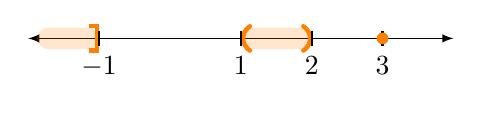
\begin{tikzpicture}[scale=0.9]
\draw[latex-latex] (-2,0) -- (4,0) ; %edit here for the axis
\draw[{[-}, ultra thick, orange] (-1,0) -- (-1.01,0);
\fill[opacity = 0.2, orange, rounded corners=1ex] (-1.88,-1ex) -- (-1, -1ex) -- (-1, 1ex) -- (-1.88,1ex) -- cycle;
\draw[shift={(-1,0)}, thick, color=black] (0pt,3pt) -- (0pt,-3pt);
\draw[shift={(-1,0)}, thick, color=black] (0pt,0pt) -- (0pt,-3pt) node[below]
{$-1$};
%
\draw[(-, ultra thick, orange] (1,0) -- (1.01,0);
\draw[-), ultra thick, orange] (2,0) -- (2.01,0);
\fill[opacity = 0.2, orange, rounded corners=1ex] (1,-1ex) -- (2, -1ex) -- (2, 1ex) -- (1,1ex) -- cycle;
\draw[shift={(1,0)}, thick, color=black] (0pt,3pt) -- (0pt,-3pt);
\draw[shift={(1,0)}, thick, color=black] (0pt,0pt) -- (0pt,-3pt) node[below]
{$1$};
\draw[shift={(2,0)}, thick, color=black] (0pt,3pt) -- (0pt,-3pt);
\draw[shift={(2,0)}, thick, color=black] (0pt,0pt) -- (0pt,-3pt) node[below]
{$2$};
%
\draw[shift={(3,0)}, thick, color=black] (0pt,3pt) -- (0pt,-3pt);
\draw[shift={(3,0)}, thick, color=black] (0pt,0pt) -- (0pt,-3pt) node[below]
{$3$};
\node at (3,0) [circle,fill,inner sep=1.5pt, color=orange]{};
\end{tikzpicture}
\end{figure}

Theres only one isolated point of $S$, $\{3 \}$.
}\end{solution}\vspace{10pt}

\begin{definition}{}{}
  $x_0$ is {\color{blue} interior } to $S$ if $x_0$ is in the interior of $S^c$. The collection of such points is the {\color{blue} exterior } of $S$.
\end{definition}\vspace{10pt}

\begin{example}{
  Let $S = (-\infty,\,-1] \cup (1,\, 2) \cup \{3\}$. Find the exterior of $S$.
}\end{example}\begin{solution}{

\begin{figure}[H]
  \centering
  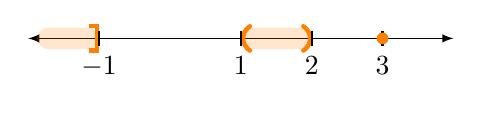
\begin{tikzpicture}[scale=0.9]
\draw[latex-latex] (-2,0) -- (4,0) ; %edit here for the axis
\draw[{[-}, ultra thick, orange] (-1,0) -- (-1.01,0);
\fill[opacity = 0.2, orange, rounded corners=1ex] (-1.88,-1ex) -- (-1, -1ex) -- (-1, 1ex) -- (-1.88,1ex) -- cycle;
\draw[shift={(-1,0)}, thick, color=black] (0pt,3pt) -- (0pt,-3pt);
\draw[shift={(-1,0)}, thick, color=black] (0pt,0pt) -- (0pt,-3pt) node[below]
{$-1$};
%
\draw[(-, ultra thick, orange] (1,0) -- (1.01,0);
\draw[-), ultra thick, orange] (2,0) -- (2.01,0);
\fill[opacity = 0.2, orange, rounded corners=1ex] (1,-1ex) -- (2, -1ex) -- (2, 1ex) -- (1,1ex) -- cycle;
\draw[shift={(1,0)}, thick, color=black] (0pt,3pt) -- (0pt,-3pt);
\draw[shift={(1,0)}, thick, color=black] (0pt,0pt) -- (0pt,-3pt) node[below]
{$1$};
\draw[shift={(2,0)}, thick, color=black] (0pt,3pt) -- (0pt,-3pt);
\draw[shift={(2,0)}, thick, color=black] (0pt,0pt) -- (0pt,-3pt) node[below]
{$2$};
%
\draw[shift={(3,0)}, thick, color=black] (0pt,3pt) -- (0pt,-3pt);
\draw[shift={(3,0)}, thick, color=black] (0pt,0pt) -- (0pt,-3pt) node[below]
{$3$};
\node at (3,0) [circle,fill,inner sep=1.5pt, color=orange]{};
\end{tikzpicture}
\end{figure}

We can write $S^c = (-1,\, 1] \cup [2,\,3)\cup(3,\,\infty)$ and then we can find the exterior of S, $(S^c)^o = (-1,\,1)\cup(2,\,3)\cup(3,\,\infty)$.
}\end{solution}\vspace{10pt}

\begin{theorem}{Limit point closure}{}
  A set $S$ is closed if and only if no point $S^c$ is a limit point of S
\end{theorem}
\begin{proof}
  Begin by proving the forward direction. If $S$ is closed, then $S^c$ is open and then for any $x_0 \in S^c \ex $ $\e$-neighborhood contained in $S^c$, hence $x_0$ cannot be a limit point.\\

  Next for the reverse direction. If no point of $S^c$ is a limit point of $S$, every point $x_0 \in S^c$ has neighborhood contained in $S^c$, hence $S^c$ is open. Therefore, $S$ is closed.
\end{proof}

\begin{corollary}
  A set is closed if and only if it contains all its limit points
\end{corollary}
What if it has no limit points? Well, it's just closed. Let us take an example:

\begin{example}{
 Take $S = \{1, 2, 3 \}$ and determine whether it closed or not.
}\end{example}\begin{solution}{


\begin{figure}[H]
  \centering
  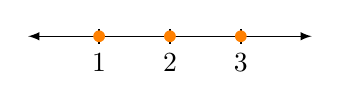
\begin{tikzpicture}[scale=0.9]
\draw[latex-latex] (0,0) -- (4,0) ; %edit here for the axis
%
\draw[shift={(1,0)}, thick, color=black] (0pt,3pt) -- (0pt,-3pt);
\draw[shift={(1,0)}, thick, color=black] (0pt,0pt) -- (0pt,-3pt) node[below]
{$1$};
\node at (1,0) [circle,fill,inner sep=1.5pt, color=orange]{};
%
\draw[shift={(2,0)}, thick, color=black] (0pt,3pt) -- (0pt,-3pt);
\draw[shift={(2,0)}, thick, color=black] (0pt,0pt) -- (0pt,-3pt) node[below]
{$2$};
\node at (2,0) [circle,fill,inner sep=1.5pt, color=orange]{};
%
\draw[shift={(3,0)}, thick, color=black] (0pt,3pt) -- (0pt,-3pt);
\draw[shift={(3,0)}, thick, color=black] (0pt,0pt) -- (0pt,-3pt) node[below]
{$3$};
\node at (3,0) [circle,fill,inner sep=1.5pt, color=orange]{};
\end{tikzpicture}
\end{figure}

You can take a deleted $\e$-neighborhood of all of these points and see that none of them are limit points. Hence the set is closed.
}\end{solution}\vspace{10pt}

\subsection{Open Coverings}

A collection $\mathcal{H}$ of open sets is an open covering of a set $S$ if every point in $S$ is contained in a set $H$ belonging to $\mathcal{H}$; that is, if $\displaystyle{S\sub \{ H : H \in \mathcal{H}\}}$

\begin{theorem}{Heine-Borel Theorem}{}
   If $\mathcal{H}$ is an open covering of a closed and bounded subset $S$ of the real line, then $S$ has an open covering $\widetilde{\mathcal{H}}$ consisting of finitely many open sets belonging to $\mathcal{H}$.
\end{theorem}

\begin{proof}
  Since S is bounded, it has supremum, $\a$, and infimum, $\b$. As $S$ is closed, we can say that $\a$ and $\b$ are in $S$. Now we shall define a couple of things:
  $$ S_t = S \cap [\a,\, t] \qquad \a \le t $$
  and let
  \begin{align*}
    F = \{ &t : \a \le t \le \b \\
    &\text{ and finitely many sets from $\mathcal{H}$ to cover $S_t$} \}
  \end{align*}
  As we know that $\displaystyle{S_\b = S}$, all we need to prove is $\displaystyle{\b \in F}$. We shall use the completeness of the reals to prove this.\\

  \noindent
  Starting with the things we know, $\displaystyle{\a \in S}$. We can then deduce that $\displaystyle{S_\a = \{ \a \}}$, which is contained in some open set, $H_\a$ from $\mathcal{H}$ as we know that $\mathcal{H}$ covers $S$, therefore $\a \in F$. Since $F$ is non-empty and bounded above by $\b$ we wish to show that the supremum, $\g$, can be seen the same as $\b$. As we definitionally know that $\g \le \b$ from $F$, it suffices to know that $\g \nless \b$. Let us consider two cases:\\

  \noindent
  \emph{Case 1:} Suppose that $\g < \b$ and $\g \notin S$. Since $S$ is closed, $\g$ is not a limit point of $S$. This means that $\ex \e > 0:$
  $$ [\g - \e,\, \g + \e] \cap S = \varnothing $$
  Then $S_{\g - \e} = S_{\g + \e}$, which can't happen, due to $\g$ being a supremum $S_{\g - \e}$ has a subcovering from $\mathcal{H}$, but $S_{\g + \e}$ wouldn't. This is a contradiction and hence if $\g \notin S$, then $\g \nless \b$.\\

  \noindent
  \emph{Case 2:} Suppose that $\g < \b$ and $\g \in S$. Then there is an open set $H_\g \in \mathcal{H}$ along with an interval, for $\e > 0$, $[\g - \e, \g + \e]$. It then follows that since $S_{\g - \e}$ has a finite covering, so does $S_{\g + \e}$. This is a contradiction from the definition of $\g$. Hence, if $\g \in S$ then $\g \nless \b$.\\

  \noindent
  So we know that $\b = \g$. Therefore $H_\b$ exists and is in $\mathcal{H}$. $H_\b$ contains $\b$ and an interval of the form, for some $\e > 0$: $[\b - \e,\, \b + \e]$. Since we know that $S_{\b - \e}$ is covered finitely by some collection: $\{ H_1,\, \dots\,, H_k \}$, then $S_\b$ is covered by some collection: $\{ H_1,\, \dots\,, H_k,\, H_\b \}$. Hence, $S_\b = S$.
\end{proof}

\begin{definition}{Compactness}{}
  A set is {\color{blue} compact }if it is closed and bounded
\end{definition}\vspace{10pt}

\begin{theorem}{Bolzano-Weirstrass Theorem}{}
  Every bounded infinite set of real numbers has at least one limit point
\end{theorem}

\begin{proof}
  It will suffice to show that a bounded nonempty set without a limit point can only contain a finite number of elements. \\

  If $S$ has no limit points, then $S$ is closed and every point, $x \in S$ has a open neighborhood, $N_x$, that only contains itself. The collection:
  $$ \mathcal{H} = \{ N_x : x \in S \} $$
  is an open covering for $S$. Heine-Borel Theorem states that $S$ can be covered by finitely many elements of $\mathcal{H}$, say $N_{x_1},\, \dots ,\, N_{x_n}$. Since these sets only depend on a finite set of points, $x_1, \, \dots \, x_n$. Then $S = \{ x_1, \, \dots \, x_n \}$ and hence, is finite.
\end{proof}


\newpage\section{Limits}
\subsection{Defining Limits}

We consider limits of real functions, that is $f: X \to \R$, with $X\sub\R$.

\noindent\begin{definition}{Limit}{}
 We say that $f(x)$ approaches the limit $L$ as $x$ approaches $x_0$, and write
 $$ \lim_{x\to x_0}{f(x)} = L$$
 if $f$ is defined on some deleted neighbourhood of $x_0$ and, for every $\e > 0$, there is a $\d > 0$ such that:
 $$ |f(x) - L| < \e $$
 if
 $$ 0 < |x - x_0| < \d $$
\end{definition}\vspace{10pt}

\begin{theorem}{Limit Uniqueness}{}
  If $\displaystyle{\lim_{x\to x_0}{f(x)}}$ exists, then it is unique, that is, if:
  $$ \lim_{x\to x_0}{f(x)} = L_1 \qquad\text{ and }\lim_{x\to x_0}{f(x)} = L_2 $$
  then $\displaystyle{L_1 = L_2}$
\end{theorem}
\begin{proof}
  Let $\ex\e>0$, such that
  $$ |f(x) - L_i| < \e \text{ if } 0 < |x - x_0| < \d_i $$
  for $i=1, 2$\\

  Now, let us look at a $|L-1 - L_2|$ and let $\d = \min(\d_1, \d_2)$.
  \begin{align*}
    |L_1 - L_2| &= |L_1 - f(x) + f(x) - L_2| \\
    &\le |L_1 - f(x)| + |L_2 - f(x)| < 2\e \\
  \end{align*}
  Given we know that $\e$ is arbitrarily small, then $|L_1 - L_2|$ is arbitrarily small and hence, $L_1 = L_2$.
\end{proof}

\begin{theorem}{Algebra of Limits}{}
  If $\lim_{x\to x_0}{f(x)} = L_1$ and $\lim_{x\to x_0}{g(x)} = L_2$, then:
  \begin{align*}
    \lim_{x\to x_0}{(f + g)} &= L_1 + L_2 \\
    \lim_{x\to x_0}{(f - g)} &= L_1 - L_2 \\
    \lim_{x\to x_0}{(fg)} &= L_1L_2 \\
    \lim_{x\to x_0}{\left(\frac{f}{g}\right)} &= \frac{L_1}{L_2} && \text{if $L_2\neq 0$}
  \end{align*}
\end{theorem}
\begin{proof}
  long and tedious
\end{proof}

\subsection{One Sided Limit}
\noindent\begin{definition}{Left-hand limits}{}
We say that $f(x)$ approaches the left-hand limit $L$ as $x$ approaches $x_0$ from the left and write:
$$ \lim_{x\to x_0^{-}}{f(x)} = L $$
if $f$ is defined on some open interval $(a, x_0)$ and, for each $\e>0, \ex \d > 0$,
$$ |f(x) - L|<\e \text{ if } x_0 - \d < x < x_0$$
\end{definition}\vspace{10pt}

\noindent{{\begin{definition}{Right-hand limit}{}
We say that $f(x)$ approaches the right-hand limit $L$ as $x$ approaches $x_0$ from the right and write:
$$ \lim_{x\to x_0^{+}}{f(x)} = L $$
if $f$ is defined on some open interval $(x_0, b)$ and, for each $\e>0, \ex \d > 0$,
$$ |f(x) - L|<\e \text{ if } x_0 < x < x_0 + \d$$
\end{definition}\vspace{10pt}

\begin{theorem}{}{}
  A function $f$ has a limit at $x_0$ $\iff$ it has right and left handed limits and they are equal.
  $$ \lim_{x\to x_0}{f(x)} = L $$
  if and only if
  $$ f(x_0-) = f(x_0+) = f(x_0) $$
\end{theorem}
\begin{proof}
  coming soon
\end{proof}

\subsection{Limits at $\pm\infty$}

\noindent\begin{definition}{Limit at infinity}{}
 We say that $f(x)$ approaches the limit $L$ as $x$ approaches $\infty$, and write:
 $$ \lim_{x\to x_0}{f(x)} = L $$
 if $f$ is defined on an interval $(a,\, \infty)$ and, for each $\e > 0$, there is a number $\b$ st,
 $$ |f(x) - L| < \e \qquad\text{if $x > \b$}$$
\end{definition}\vspace{10pt}

\noindent\begin{definition}{Left infinite limit}{}
 We say $f(x)$ approaches $\infty$ as $x$ approaches $x_0$ from the left, and write:
 $$ f(x_0-) = \infty $$
 if $f$ is defined on an interval $(a, x_0)$ and, for each real number $M$, there is a $\d > 0$ such that:
 $$ f(x) > M \text{ if } x_0 - \d < x < x_0 $$
\end{definition}\vspace{10pt}

NB! When we say a limit exists, we mean that it is finite, i.e. not $\pm\infty$. If it is, we can say it exists in the extended reals.\\

Also with infinite limits, we know that the `Uniqueness of Limits' and the `Algebra of Limits' are also valid when $x_0$ are replaced by $\pm\infty$.\\

The `Alegbra of Limits' rules are also valid if $L_1,L_2 = \infty$ provided the RHS are not indeterminant forms.

\subsection{Monotonics}
\noindent\begin{definition}{Monotonicity}{}
A function $f$ is {\color{blue} nondecreasing }on an interval $I$ if:
$$ f(x_1) \le f(x_2) \quad\text{if }x_1,x_2\in I \text{ and }x_1<x_2$$
or {\color{blue} nondecreasing }if,
$$ f(x_1) \ge f(x_2) \quad\text{if }x_1,x_2\in I \text{ and }x_1<x_2$$
We further define that if the `$\le$' can be replaced with a `$<$', then $f$ is strictly monotonic on $I$
\end{definition}\vspace{10pt}

\begin{theorem}{}{}
  Suppose that $f$ is monotonic on $(a,\, b)$ and define
  $$ \a = \inf_{a<x<b}{f(x)} \text{ and } \sup_{a<x<b}{f(x)} $$
  \begin{enumerate}
    \item If $f$ is nondecreasing, then $f(a+)=\a$ and $f(b-)=\b$
    \item If $f$ is nonincreasing, then $f(a+)=\b$ and $f(b-)=\a$.
    \item If $a<x_0<b$, then $f(x_0+)$ and $f(x_0-)$ exist and are finite; moreover;
    $$ f(x_0-) \le f(x_0) \le f(x_0+) $$
    if $f$ is nondecreasing, and
    $$ f(x_0-)\ge f(x_0) \ge f(x_0+) $$
    if $f$ is nonincreasing
  \end{enumerate}
\end{theorem}
\begin{proof}
  Too long and tedious to typeset
\end{proof}

\newpage
\newpage\section{Continuity}
Now we have defined limits, we can now define continuity.\\

\noindent\begin{definition}{Continuity at $x_0$}{}
 We say that $f$ is continuous at $x_0$ if $f$ is defined on an open interval $(a, b)$ containing $x_0$ and that $\lim_{x\to x_0}{f(x)} = f(x_0)$.
\end{definition}\vspace{10pt}

\noindent\begin{definition}{Left continuity at $x_0$}{}
  We say $f$ is continuous from the left at $x_0$ if $f$ is defined on an open interval $(a, x_0)$ and $f(x_0-) = f(x_0)$.
\end{definition}\vspace{10pt}

\noindent\begin{definition}{Right Continuity at $x_0$}{}
  we say $f$ is continuous from the right at $x_0$ if $f$ is defined on an open interval $(x_0,\, b)$ and $f(x_0+) = f(x_0)$.
\end{definition}\vspace{10pt}

\begin{theorem}{}{}
  A function $f$ is continuous at $x_0$ if and only if $f$ is defined on an open interval $(a, b)$ containing $x_0$ and for each $\e>0$ there is a $\d>0$ st,
  \begin{equation}
    |f(x) - f(x_0)| < \e
  \end{equation}
  whenever $|x - x_0| < \d$
\end{theorem}

\begin{theorem}{}{}
  A function $f$ is continuous from the right at $x_0$ if and only if $f$ is defined on an interval $[x_0,\, b)$ and for each $\e > 0\ex\d > 0$ st (1) holds whenever: $\displaystyle{x_0 \le x < x_0 + \d}$
\end{theorem}

\begin{theorem}{}{}
  A function $f$ is continuous from the left at $x_0$ if and only if $f$ is defined on an interval $(a, x_0]$ and for each $\e > 0\ex\d > 0$ st (1) holds whenever: $\displaystyle{x_0 - \d < x \le x_0}$
\end{theorem}

Note that $f$ is continuous if and only if $f(x_0-) = f(x_0+) = f(x_0)$.\\

\noindent\begin{definition}{Continuous on a set}{}
 A function $f$ is continuous on an open interval $(a,\, b)$ if it is continuous at every point in $(a,\, b)$. If, in addition,
 \begin{equation}
   f(b-)=f(b)
 \end{equation}
 or
 \begin{equation}
   f(a+) = f(a)
 \end{equation}
 then $f$ is continuous on $(a,\,b]$ or $[a,\,b)$ respectively. If both are true then $f$ is continuous on $[a,\,b]$.
\end{definition}\vspace{10pt}
More generally, if $S$ is a subset of $D_f$ consisting of finitely or infinitely many disjoint intervals, then $f$ is continuous on $S$ if $f$ is continuous on every interval in $S$. (From here on, if we say ``$f$ is continuous on $S$'' we mean $S$ is a set of this kind.).

\subsection{Discontinuities}

\noindent\begin{definition}{Piecewise Continuity}{}
  $f$ is {\color{blue} piecewise continuous }on $[a,\,b]$ if
  \begin{enumerate}
    \item $\ex f(x_0+)\forall x_0\in[a,\,b)$
    \item $\ex f(x_0-)\forall x_0\in(a,\,b]$
    \item $f(x_0+) = f(x_0-) = f(x_0)$ for all but finitely many points $x_0\in (a,\,b)$
  \end{enumerate}
  If (3) fails to hold at some $x_0$ in $(a,\,b)$, $f$ has a {\color{blue}  jump discontinuity}.
\end{definition}\vspace{10pt}

\noindent\begin{definition}{Removable discontinuity}{}
Let $f$ be defined on a deleted neighborhood of $x_0$ and be discontinuous (perhaps even undefined) at $x_0$. We say that $f$ has a removable discontinuity at $x_0$ if $\lim_{x\to x_0}{f(x)}$ exists. In
this case, the function
$$g(x) = \begin{cases}
  f(x) & \text{if $x\in D_f$ and $x\neq x_0$} \\
  \lim_{x\to x_0}{f(x)} & \text{ if $x = x_0$}\\
\end{cases} $$
is continuous at $x_0$.
\end{definition}\vspace{10pt}

\subsection{Continuity Arithmetic}
\begin{theorem}{}{}
  If $f$ and $g$ are continuous on a set $S$, then so are $f + g$, $f - g$ and $fg$. So is $\displaystyle{\frac{f}{g}}$ given $g\neq 0$ at $x_0$.
\end{theorem}

\begin{theorem}{}{}
  Suppose that $g$ is continous at $x_0$, $g(x_0)$ is an interior point of $D_f$ and $f$ is continuous at $g(x_0)$. Then $f\circ g$ is continuous at $x_0$.
\end{theorem}
\begin{figure}[H]
  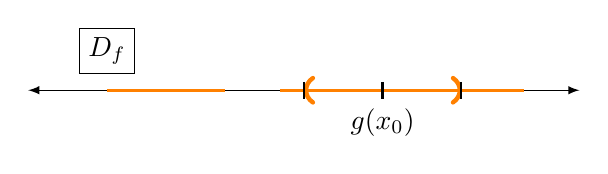
\begin{tikzpicture}
    \draw[latex-latex] (-3.5,0) -- (3.5,0) ; %edit here for the axis
    \draw[(-, ultra thick, orange] (0,0) -- (0.01,0);
    \draw[{-)}, ultra thick, orange] (2,0) -- (2.01,0);
    %\fill[opacity = 0.2, blue,rounded corners=1ex] (0,-1ex) -- (2, -1ex) -- (2, 1ex) -- (0,1ex) -- cycle;
    \draw[very thick, color=orange] (-0.3,0) -- (2.8,0);
    \draw[very thick, color=orange] (-2.5,0) -- (-1,0);
    \node[draw] at (-2.5, 0.5) {$D_f$};
    %
    \draw[shift={(0,0)}, thick, color=black] (0pt,3pt) -- (0pt,-3pt);
    \draw[shift={(0,0)}, thick, color=black] (0pt,0pt) -- (0pt,-3pt);
    %
    \draw[shift={(2,0)}, thick, color=black] (0pt,3pt) -- (0pt,-3pt);
    \draw[shift={(2,0)}, thick, color=black] (0pt,0pt) -- (0pt,-3pt);
    %
    \draw[shift={(1,0)}, thick, color=black] (0pt,3pt) -- (0pt,-3pt);
    \draw[shift={(1,0)}, thick, color=black] (0pt,0pt) -- (0pt,-3pt) node[below]
    {$g(x_0)$};
  \end{tikzpicture}
\end{figure}

So the above theorem is saying that we must have some $(g(x_0) - \e,\, g(x_0) + \e) \sub D_f$ or even that; $\displaystyle{\lim_{x\to x_0}{f(g(x))} = f(g(x_0))}$.

\begin{proof}
  Suppose $\e>0$, since $g(x_0)\in D_f^o$ and $f$ is continous at $g(x_0), \ex\d_1>0$ st, $f(t)$ is defined and
  \begin{equation}
    |f(t) - f(g(x_0))|<\e \text{ if } |t - g(x_0)| < \d_1
  \end{equation}
  Since $g$ is continuous at $x_0$, $\ex\d_2>0$ st, $g(x)$ is defined (why?) and
  \begin{equation}
    |g(x) - g(x_0)| < \d_1 \text{ if } |x - x_0|<\d_2
  \end{equation}
  Then (4) and (5) imply that,
  $$ |f(g(x)) - f(g(x_0))| < \e \text{ if } |x - x_0| < \d_2 $$

\end{proof}

\newpage
\newpage\section{Boundedness}

\noindent\begin{definition}{Bounded Below}{}
 A funtion $f$ is bounded below on a set $S$ if theres an $m\in\R$
 $$ f(x) \geq m \qquad\forall x\in S $$
 In this case,
 $$ V = \{ f(x) : x\in S\} $$
 has an infimum, $\a$, and we write,
 $$ \a = \inf_{x\in S}{f(x)} $$
 If $\ex x_1\in S$, such that $f(x_1) = \a$, then we say that $\a$ is the minimum of $f$ on $S$ and write:
 $$ \a = \min_{x\in S}{f(x)} $$
\end{definition}\vspace{10pt}

\noindent{{\begin{definition}{Bounded Above}{}
 $f$ is bounded above on $S$, if $\ex M\in\R$, such that, $f(x) \le M \qquad \forall x\in S$. Then we can write;
 $$ \b = \sup_{x\in S}{f(x)} $$
 If $\ex x_2\in S$, such that $f(x_2) = \b$, then we say that $\b$ is the minimum of $f$ on $S$ and write:
 $$ \b = \max_{x\in S}{f(x)} $$
\end{definition}\vspace{10pt}

\noindent\begin{definition}{Bounded}{}
  If $f$ is both bounded below and bounded above on a set $S$, then $f$ is bounded on $S$.
\end{definition}\vspace{10pt}
\begin{theorem}{Boundedness Theorem}{}
  If $f$ is continuous on a finite closed interval $[a,\, b]$, then $f$ is bounded on $[a,\,b]$
\end{theorem}
\begin{figure}[H]
  \centering
  \begin{tikzpicture}[declare function={f(\x)=0.3*(\x-3.5)^3-\x+7;a=1;b=6;c=4.94; t = 3;}] %starts and declares the function
   \draw[-stealth] (-0.5,0) -- (6.5,0); % draw x axis
   \draw[-stealth] (0,-0.5) -- (0,6.5); % draw y axis
   \draw[blue] plot[smooth,domain={a}:{b}] ({\x},{f(\x)}); %draws function
   \foreach \X in {a,b,t}
   {\draw[dashed] (\X,0) node[below]{$\X$} |- (0,{f(\X)}) node[left] {$f(\X)$};} %plots points and draws dashes
   % \e-neighbourhood code
   \draw[(-, ultra thick, red] (2.75,0) -- (2.76,0);
   \draw[{-)}, ultra thick, red] (3.25,0) -- (3.26,0);
   \draw[ultra thick, red] (2.75,0) -- (3.25,0);
   % \d-neighbourhood
   \draw[(-, ultra thick, red] (0, {f(3)-0.25}) -- (0, {f(3)-0.24});
   \draw[{-)}, ultra thick, red] (0, {f(3)+0.25}) -- (0, {f(3)+0.26});
   \draw[ultra thick, red] (0, {f(3)-0.25}) -- (0, {f(3)+0.25});
   %
   \node at (a,{f(a)}) [circle,fill,inner sep=1.5pt, color=blue]{};
   \node at (b,{f(b)}) [circle,fill,inner sep=1.5pt, color=blue]{};
  \end{tikzpicture}
  \caption{Assume $f$ is bounded, it curves again, I promise...}
\end{figure}
\begin{proof}
  Suppose we take a $t\in[a,\,b]$. Since $f$ is continuous at $t $  $\ex $ an open interval, $t\in I_t$, st,
  \begin{equation*}
  |f(x) - f(t)|<1 \qquad\text{if $x\in I_t\cap[a,\,b]$}\tag{$*$}
\end{equation*}
  The collection $\displaystyle{\mathcal{H} = \{ I-t : a \le t \le b \}}$ is an open cover of $[a,\, b]$. Since, $[a,\, b]$ is compact, then by the Heine-Borel theorem, there exists a finite sub-cover made up of intervals $I_{t_1},\,\dots,\,I_{t_n}$. By ($*$), taking $t = t_i$, then,
  $$ |f(x) - f(t_i)|< 1 \qquad\text{if $x\in I_{t_i}\cap[a,\,b]$} $$
  Therefore,
  \begin{align*}
    |f(x)| &= |f(x) - f(t_i) + f(t_i)| \\
    &\le |f(x) - f(t_i)| + |f(t_i)| \\
    &\le 1 + |f(t_i)|\qquad \text{if $x\in I_{t_i}\cap[a,\,b]$} \tag{$**$}\\
  \end{align*}
Let $\displaystyle{M = 1 + \max_{1\le i\le n}{|f(t_i)|}}$ and since,\\ $\displaystyle{[a,\,b]\sub \bigcup_{i=1}^n{I_{t_i}\cup[a,\,b]}}$, then apply ($**$) and then
$$ |f(x)| \le M \qquad\forall x\in[a,\,b] $$
\end{proof}

\begin{theorem}{Extreme value Theorem}{}
  Suppose that $f$ is continuous on a finite closed interval, $[a, b]$. Let,
  $$ \a = \inf_{a\le x\le b}{f(x)}\text{ and } \b =\sup_{a\le x\le b}{f(x)} $$
  Then $\a$ and $\b$ are respectively the minimum and maximum of $f$ on $[a,\,b]$; that is there are points $x_1$ and $x_2$ in $[a,\,b]$ such that;
  $$ f(x_1) = \a \qquad f(x_2) = \b $$
\end{theorem}
\begin{proof}
  We'll show that $x_1$ exists first. Suppose for a contradiction, that there is no point $x_1 \in [a,\,b], f(x_1) = \a$. Then for $f(t) > \a\quad \forall t \in [a,\,b]$
  $$ f(t) > \frac{f(t) + \a}{2} > \a $$
  Since, $f$ is continuous at $t$, there is an open interval $I_t$ about the point $t$, st,
  $$ f(x) > \frac{f(t) + \a}{2} \qquad x\in I_t\cap[a,\, b] $$
  Then, the collection of $\displaystyle{\mathcal{H} = \{ I_t: a\le x \le b\}}$ is an open covering of $[a, \, b]$. Since $[a, \, b]$ is compact, the Heine-Borel theorem implies that there is a finite sub-covering using some open intervals $I_{t_1},\,\dots,\,I_{t_n}$ around $t_1,\,\dots,\,t_n$. Now we define:
  $$ \a_1 = \min_{1\le i \le n}{\frac{f(t_i) + \a}{2}} $$
  Then $f(t) > \a \,\forall \,t \in \bigcup_{i=1}^n{I_{t_i}\cap[a,\,b]} = [a,\,b]$, so we now have $a_1 >\a$ and hence a contradiction. So $f(x_1) = \a$ for some $x_1\in [a,\,b]$.\\

  \noindent
  To complete the proof, show that $x_2$ exists. Suppose for a contradiction, that there is no point $x_2 \in [a,\,b], f(x_2) = \b$. Then for $f(t) < \b\quad \forall t \in [a,\,b]$
  $$ f(t) < \frac{f(t) + \b}{2} < \b $$
  Since, $f$ is continuous at $t$, there is an open interval $I_t$ about the point $t$, st,
  $$ f(x) < \frac{f(t) + \b}{2} \qquad x\in I_t\cap[a,\, b] $$
  Then, the collection of $\displaystyle{\mathcal{H} = \{ I_t: a\le x \le b\}}$ is an open covering of $[a, \, b]$. Since $[a, \, b]$ is compact, the Heine-Borel theorem implies that there is a finite sub-covering using some open intervals $I_{t_1},\,\dots,\,I_{t_n}$ around $t_1,\,\dots,\,t_n$. Now we define:
  $$ \b_1 = \max_{1\le i \le n}{\frac{f(t_i) + \b}{2}} $$
  Then $f(t) < \b \,\forall \,t \in \bigcup_{i=1}^n{I_{t_i}\cap[a,\,b]} = [a,\,b]$, so we now have $\b <\b_1$ and hence a contradiction. So $f(x_2) = \b$ for some $x_2\in [a,\,b]$.
\end{proof}
\begin{figure}[H]
  \centering
  \begin{tikzpicture}[declare function={f(\x)=0.3*(\x-3.5)^3-\x+7;a=1;b=6;}] %starts and declares the function
   \draw[-stealth] (-0.5,0) -- (6.5,0); % draw x axis
   \draw[-stealth] (0,-0.5) -- (0,6.5); % draw y axis
   \draw[blue] plot[smooth,domain={a}:{b}] ({\x},{f(\x)}); %draws function
   \foreach \X in {a,b}
   {\draw[dashed] (\X,0) node[below]{$\X$} |- (0,{f(\X)}) node[left] {$f(\X)$};} %plots points and draws dashes
   \draw[dashed, thick, green] (3,0) node[below]{$c$} |- (0,{f(3)}) node[left] {$\mu$};
   \draw[dotted, thick, orange] (1, {f(1)}) -- (6, {f(6)});
   % endpoints of the graph
   \node at (a,{f(a)}) [circle,fill,inner sep=1.5pt, color=blue]{};
   \node at (b,{f(b)}) [circle,fill,inner sep=1.5pt, color=blue]{};
  \end{tikzpicture}
\end{figure}
\begin{theorem}{Intermediate Value Theorem}{}
  Suppose that $f$ is continuous on $[a,\, b]$, $f(a)\neq f(b)$, and $\mu$ is between $f(a)$ and $f(b)$. Then $f(c) = \mu$, for some $c\in [a,\, b]$
\end{theorem}
\begin{proof}
  Suppose that $f(a) < \mu < f(b)$. The set,
  $$ S = \{ x : a \le x \le b \text{ and }f(x)\le\mu  \} $$
  is bounded and is non-empty. Let $c = \sup S$. We will show that $f(c) = \mu$. If $f(c) > \mu$, then $c > a$ and since $f$ is continuous at $c$, $\ex\e>0$,st,
  $$ f(x) > \mu \qquad\text{ if }c - \e < x \le c $$
  Therefore, $c - \e$ is an upper bound for $S$, contradicting the definition of $c$.\\
  If $f(c) < \mu$, then $c < b$ and $\ex\e>0$, st,
  $$ f(x) < \mu \text{ for } c \le x < c + \e $$
  so $c$ is not an upper bound for $S$, which again contradicts the definition of $c$. \\
  Therefore $f(c) = \mu$. The proof for $f(b) < \mu < f(a)$ is simply obtained by applying the above to the function $-f$.
\end{proof}

\subsection{Monotonics 2: God what a mess}


\end{document}
